\chapter{Búsqueda en anchura (BFS)}
La BFS es similar a la DFS, en el sentido que explora todos los estados a los que se puede llegar a partir uno inicial.

Pero la diferencia es que esto los explora un orden diferente.

La DFS lo que hace es en un estado, explora totalmente lo que ofrezca una transición lo más profundo que puede hasta ya no poder explorar más y luego  da vuelta atrás para ver transiciones que dejo pendiente.

En cambio, la BFS lo que hace es que hace es primero explorar el estado inicial, luego todos los estados que fueron descubiertos desde el inicial, luego los que fueron descubiertos en el paso anterior y así seguir.

Mostremos un diagrama del comportamiento de la BFS, en el diagrama los estados son representados por círculos. Si han sido explorados los marcamos de gris, pero si están en la lista por explorar, los dejamos blancos. Las flechas representan las transiciones. Finalmente, los estados están enumerados en el orden que fueron alcanzados por la BFS.

Iniciamos explorando el estado inicial, 1 y poniendo los estados que alcanza en la lista por explorar.

\begin{center}
	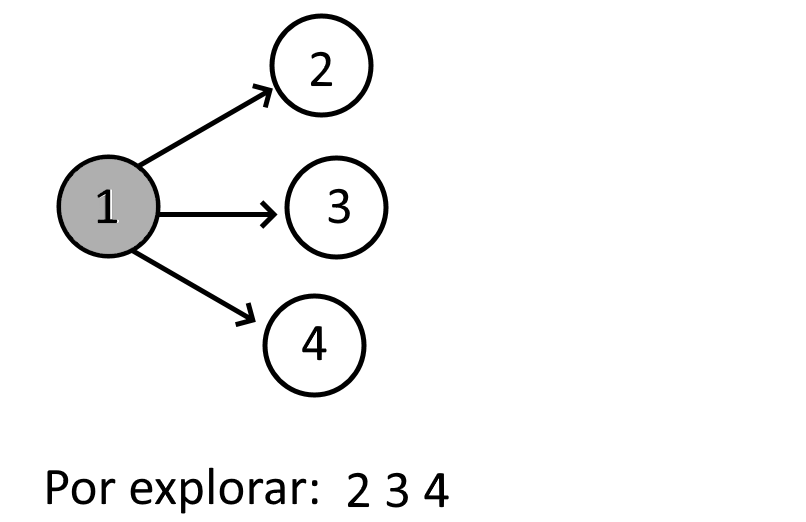
\includegraphics[scale=0.35]{bfs1}
\end{center}

Y luego para cada una de esos estados los exploramos también y los nuevos que encontremos los vamos poniendo en la lista de "estados por explorar". 

\begin{center}
	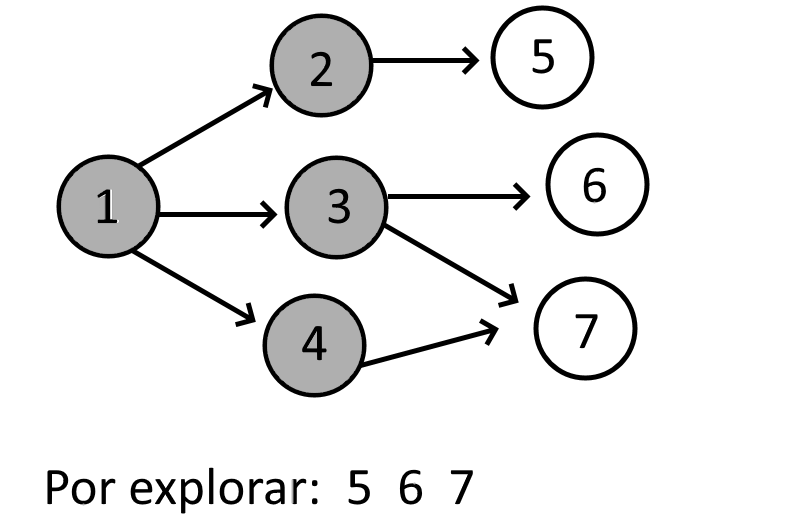
\includegraphics[scale=0.35]{bfs2}
\end{center}

De esta forma, comenzamos visitando todos los lugares alcanzables con una transición, luego dos transiciones, después tres, cuatro, cinco y  así sucesivamente.

Y precisamente, este orden en el que exploramos nos da una buena ventaja. A todo estado llegamos con la menor cantidad de transiciones posibles. Lo cual podemos guardar ya que esto llega a ser información útil para muchos problemas.

Entonces, el pseudocódigo de una BFS se ve de la siguiente forma

\begin{minipage}{\linewidth}
\begin{lstlisting}
bool visitado[];
int no_transiciones[];
explorando[];
porExplorar[];

void BFS(inicio) {
	explorando[0]=inicio;
	visitado[inicio]=true;
	no_transiciones[inicio]=0;
	int numExp=1;//No de elemntos en la lista explorando
	int numPorExp=0;//No de elemntos en la lista porExplorar
	//mientras explorando no este vacio
	while (numExp>0) {
		//Encontar los estados alcanzables desde explorando
		for (int i =0; i < numExp; i++) {
			estado= explorando[i];
			for (transicion del estado) {
				if (visitado[transicion]==false) {
					no_transiciones[transicion]=
						1+no_transiciones[estado];
					visitado[transicion]=true;
					porExplorar[numPorExp]=transicion;
					numPorExp++;
				}
			}
		}
		//Pasar porExplorar a explorando para la siguiente iteracion
		for (int i=0; i < numPorExp; i++) 
			explorando[i]=porExplorar[i];
		numExp=numPorExp;
		numPorExp=0;
	}
}
\end{lstlisting}
\end{minipage}

Como ya es de costumbre, veamos un ejemplo para entender esto.
\section*{Ejemplo: Dos operaciones}
Javier tiene una calculadora un poco peculiar. Esta muestra un número \(x\) en pantalla y tiene dos botones.

\begin{plimits}
	\item El primer botón le suma \(a\) al valor de \(x\).
	\item El segundo botón le  suma \(\frac{x}{b}\) a \(x\), pero solo puede ser presionado cuando \(x\) sea un múltiplo de \(b\).
\end{plimits}

Ahora Javier se pregunta cuantas veces debe presionar un botón para que el valor \(x\) se convierta en \(y\).

\textbf{Entrada}\\
La entrada constará de cuatro enteros: \(x\), \(y\), \(a\) y \(b\). El valor inicial de la calculadora, el valor deseado, y el valor de \(a\) y \(b\) para los botones.

\textbf{Salida}\\
Imprime un entero que sea la cantidad de pulsaciones mínima para convertir \(x\) a \(y\). Si es imposible pasar de \(x\) a \(y\) imprime \(-1\).

\textbf{Ejemplo}\\
\begin{casebox3}
	\ecase{	1 20 4 5}{6}
	{	Presiona el primer botón, ahora tienes 5.\\		
		Usa el segundo, ahora vale 6.\\
		Pulsa el primer botón, obtienes 10.\\
		Utiliza el segundo para tener 12.\\
		Usa el primer botón, obtén 16.\\
		Termina con el primero, llegamos a 20.
	}
	\ecase{	1 32 3 2}{-1}
	{	Es imposible obtener 32.
	}
\end{casebox3}

\textbf{Límites}
\begin{plimits}
	\item \(1\leq x,y,a,b \leq 10^5\)
\end{plimits}

ENLACE: TODO

\subsection*{Solución}
Entonces, en este problema nos piden la mínima cantidad de operaciones para pasar de \(x\) al valor de \(y\).

Recordemos que la BFS es perfecta para esta situaciones, pues calcula la mínima cantidad de transiciones para pasar de un estado inicial a todos los demás, incluyendo \(y\).

Para esto haremos una BFS que use de estados el número de la calculadora y de transiciones los botones. Esta explorará todas las operaciones desde \(x\) hasta llegar a \(y\).

Esto se verá:

\begin{minipage}{\linewidth}
\begin{lstlisting}
bool visitado[100005];
int distancia[100005];
int explorando[100005], porExplorar[100005];
int bfs(int x, int y, int a, int b) {
	explorando[0]=x;
	visitado[x]=true;
	distancia[x]=0;
	int numExp=1, numPorExp=0;
	while (numExp>0) {
		for (int i=0;i<porExp; i++) {
			int actual=explorando[i];
			if (actual==y)
				return distancia[x];
			
			int siguiente= actual+a;
			if (siguiente <= y && visitado[siguiente]==false) {
				visitado[siguiente]=true;
				distancia[siguiente]=1+distancia[actual];
				porExplorar[numPorExp++]=siguiente;
			}
			siguiente=actual+actual/b;
			if (siguiente <= y && actual%b ==0 && visitado[siguiente]==false) {				
				visitado[siguiente]=true;
				distancia[siguiente]=1+distancia[actual];				
				porExplorar[numPorExp++]=siguiente;
			}
		}
		for (int i=0; i<numPorExp; i++)
			explorando[i]=porExplorar[i];
		numExp=numPorExp; 
		numPorExp=0;
	}
	return -1;
}
\end{lstlisting}
\end{minipage}

\section{Complejidad}
La complejidad de una BFS es sencillamente de calcular. Veamos que cada estado es colocado una sola vez dentro de la cola y por lo tanto, explorado una sola vez.

Por lo tanto, cada transición también es visitada una única vez, cuando su estado correspondiente sea visitado.

Esto provoca que la complejidad de la BFS sea \(O(V+E)\), donde \(V\) es la cantidad de estados y \(E\) es el número de transiciones.

En el ejemplo 5.1, la cantidad de estados son a lo más \(y\) y a lo más tenemos dos transiciones por estado, por lo que la complejidad es \(O(V+E)=O(y+2y)=O(y)\).\\

\section*{Ejemplo: OMI-98 Explorador II}

Un explorador tiene que decidir donde construir un camino para llegar de un punto \(A\) a un punto \(B\). 

Para auxiliarse el explorador ha hecho un mapa con los obstáculos que existen. Cuadriculó su mapa y quiere un camino que pase por el menor número de cuadros. El camino sólo puede ir de un cuadro a otro si tienen un lado en común, es decir, no puede avanzar en diagonal, y no puede pasar por un cuadro que contenga un obstáculo. 

Cada cuadro del mapa se identifica por sus coordenadas, primero la fila y después la columna. Las filas están numerados de arriba hacia abajo iniciando con el \(0\). Las columnas están numeradas de izquierda a derecha iniciando con el \(0\).

Escribe un programa que dado un mapa con obstáculos encuentre el menor número de cuadros por los que debe pasar un camino que vaya del punto \(A\) al punto \(B\), incluyendo a los cuadros que contienen a \(A\) y a \(B\).

\textbf{Entrada}\\
En la primera línea los enteros \(N\) y \(M\) el número de filas y columnas del mapa. En cada una de las siguientes.

En las siguientes \(N\) líneas hay \(M\) enteros que pueden ser \verb|0| ó \verb|1|. Es \verb|0| si no hay obstáculo en el cuadro correspondiente y \verb|1| si lo hay.

En la siguiente línea (la penúltima) la fila y columna del punto \(A\).

En la última línea la fila y columna del punto \(B\).

\textbf{Salida}\\
En la primera linea el número de cuadros por los que pasa un camino mínimo entre \(A\) y \(B\)

\textbf{Ejemplo}\\
\begin{casebox2}
	\scase{
		4 5\\
		0 1 0 0 0\\
		0 0 1 1 0\\
		0 1 0 0 0\\
		0 0 0 0 0\\
		3 1\\
		0 2	
	}{9}
\end{casebox2}

\textbf{Límites}
\begin{plimits}
	\item \(1 \leq N, M\leq 750\)
\end{plimits}

ENLACE TODO

\subsection*{Solución}
Anteriormente vimos una solución con Podas para este problema con complejidad \(O((NM)^2)\), pero esto no es suficiente para este problema.

Claramente, podemos hacer una BFS donde los estados sea cada punto de la cuadricula y que cuente cuantos pasos necesito para llegar a \(B\) iniciando desde \(A\).

Entonces nuestros estados serán descritos con dos valores \(f\) y \(c\), la fila y columna. Pero hasta ahora la BFS que vimos usa solo un número como valor, piensa en como adaptarla para que se puedan usar estados que usen dos valores y trata de resolverlo antes.

\subsubsection*{Usando dos valores}
La forma de adaptar la BFS que vimos para funcionar con esto es bastante sencillo. Lo único que necesitamos hacer es que en vez de introducir un valor a la lista porExplorar, agregamos dos por cada estado.

De forma que si en porExplorar tenemos tres casillas, esta lista se vería \{f1, c1, f2, c2, f3, c3\}

Entonces, lo que podemos hacer es realizar la bfs. El código quedará aproximadamente:

\begin{minipage}{\linewidth}
\begin{lstlisting}
bool visitado[755][755];
int distancia[755][755];
int BFS(int Afila, int Acolumna) {
	explorar[0]=Afila; explorar[1]=Acolumna;
	visitado[Afila][Acolumna]=true;
	int numExp=2; int numPorExp=0;
	int transicionesI[4]   ={1,-1,0,0};
	int transicionesJ[4]={0,0,1,-1};
	for (int c =0; c < numExp; c+=2) {
		int i = explorando[c];
		int j = explorando[c+1];
		if (i==Bfila && j==Bcolumna) return distancia[i][j];
		for (int tr =0; tr < 4; tr++) {
			int ni= i+transicionesI[tr];
			int nj= j+transicionesJ[tr];
			if (0<=ni && ni < N && 0 <=nj && nj<M) {
				if (mapa[ni][nj]==0 && !visitado[ni][nj]) {
					visitado[ni][nj]=true;
					distancia[ni][nj]=1+distancia[i][j];
					porExplorar[numPorExp]=ni; //Agrega la coordenada ni
					porExplorar[numPorExp+1]=nj; //Agrega la coordenada nj
					numPorExp+=2;
				}
			}
		}
		[...]
	}
}
\end{lstlisting}
\end{minipage}

\section*{Problemas de práctica}
\addcontentsline{toc}{section}{Problemas de práctica}

\begin{exercise}
	\problema{Two Buttons}{\codeforceslink{520}{B}}
	Traduccion: TODO
\end{exercise}

\begin{exercise}
	\problema{Camino mas corto en matriz}{TODO}
\end{exercise}

\begin{exercise}
	\problema{Volcan}{\omegauplink{Volcan}}
\end{exercise} 

\begin{exercise}
	\problema{IOI 1994 - Relojes}{\omegauplink{relojes}}
\end{exercise}

\begin{exercise}
	\problema{OMI 2020 - Ovejas}{\omegauplink{omi-2020-ovejas}}	
\end{exercise}

